\chapter{Los descomponedores y el suelo}\label{ch:g6:decomposers-and-soil}

Todos los otoños, el bosque suelta una alfombra espesa de \omterm{def:g1:plants-around-us:parts}{hojas} ---
toneladas por hectárea. Y sin embargo, recorre ese mismo bosque cada
primavera y no vadearás ningún mar creciente de hojarasca: la alfombra
vuelve a estar fina, año tras año. Alguien se está comiendo a los
muertos del bosque. Este capítulo baja al \omterm{def:g6:decomposers-and-soil:soil}{suelo} a conocer a los
comensales --- y a cerrar, por fin, el círculo de la materia.

\section{El suelo está vivo}

\begin{definition}[Suelo]\label{def:g6:decomposers-and-soil:soil}
El \emph{suelo}\index{suelo} es la \omterm{def:g1:the-five-senses:sense}{piel} viva de la Tierra: una mezcla
de granos \emph{minerales} (roca molida, de la arena a la arcilla),
restos \emph{orgánicos} en todas las fases de la \omterm{prop:g6:decomposers-and-soil:decomposition}{descomposición}, agua,
aire --- y una población enorme de \omterm{def:g6:exploring-our-environment:components}{seres vivos}. Su capa superior y
oscura, la más rica en materia descompuesta, es la capa de
\emph{humus}\index{humus} que tanto aprecian los hortelanos.
\end{definition}

\begin{example}[Un puñado, censado]\label{ex:g6:decomposers-and-soil:handful}
Un puñado de \omterm{def:g6:decomposers-and-soil:soil}{suelo} de bosque, clasificado sobre una bandeja blanca:
granos minerales; hilos de \omterm{def:g1:plants-around-us:parts}{raíz}; medias \omterm{def:g1:plants-around-us:parts}{hojas}, \omterm{def:g3:bones-and-muscles:skeleton}{esqueletos} de \omterm{def:g1:plants-around-us:parts}{hoja} y
migas negras --- \omterm{def:g6:plants-are-producers:matter}{materia orgánica} camino de abajo; y el censo --- una
lombriz, dos cochinillas, un milpiés, colémbolos blancos diminutos,
fieltros de \omterm{def:g6:decomposers-and-soil:decomposers}{hongo} finos como hilos. Y la bandeja solo enseña lo
visible: un solo gramo de \omterm{def:g6:decomposers-and-soil:soil}{suelo} alberga más \omterm{def:g6:exploring-our-environment:components}{seres vivos} demasiado
pequeños para verlos que personas hay en una gran ciudad.
\end{example}

\begin{definition}[Descomponedores]\label{def:g6:decomposers-and-soil:decomposers}
Los \emph{descomponedores}\index{descomponedor} son los \omterm{def:g6:exploring-our-environment:components}{seres vivos}
que se alimentan de \emph{\omterm{def:g6:plants-are-producers:matter}{materia orgánica} muerta} --- \omterm{def:g1:plants-around-us:parts}{hojas} caídas,
madera muerta, excrementos, cadáveres:
\begin{itemize}
  \item la cuadrilla visible: lombrices, cochinillas, milpiés,
        colémbolos, larvas de mosca, escarabajos peloteros;
  \item los \emph{hongos}\index{hongo}: mohos y setas, cuyo cuerpo que
        se alimenta es un fieltro de hilos blancos extendido por el
        \omterm{def:g6:decomposers-and-soil:soil}{suelo} y por la madera muerta --- la seta del
        \cref{exo:g1:living-or-not:10} es solo su \omterm{prop:g3:flowers-fruits-seeds:transform}{fruto};
  \item y, rematando todos los trabajos, vida del \omterm{def:g6:decomposers-and-soil:soil}{suelo} demasiado
        pequeña para verla --- los desmontadores finales.
\end{itemize}
Son los trabajadores en la sombra de la
\cref{def:g5:food-webs:roles}, a los que se les prometió un capítulo
propio: es este.
\end{definition}

\section{La descomposición: de lo orgánico a lo mineral}

\begin{proposition}[Qué hace la descomposición]\label{prop:g6:decomposers-and-soil:decomposition}
La \emph{descomposición}\index{descomposición} es la alimentación de
los \omterm{def:g6:decomposers-and-soil:decomposers}{descomponedores}, y su resultado es lo contrario del oficio de las
\omterm{def:g5:food-webs:roles}{productoras}: la materia \emph{orgánica} muerta se desmonta, fase a fase
y comensal a comensal, hasta que su sustancia vuelve al mundo
\emph{mineral} --- \omterm{def:g6:decomposers-and-soil:soil}{humus} desmenuzado, después \omterm{prop:g4:what-plants-need:needs}{sales minerales} disueltas
en el agua del \omterm{def:g6:decomposers-and-soil:soil}{suelo} y gas devuelto al aire. La alfombra de otoño se
convierte, para la primavera, exactamente en lo que beben las \omterm{def:g1:plants-around-us:parts}{raíces}
(\cref{prop:g4:what-plants-need:needs}).
\end{proposition}
\admitted

\begin{example}[El último año de la hoja]\label{ex:g6:decomposers-and-soil:leaf}
Sigue una \omterm{def:g1:plants-around-us:parts}{hoja} de roble hacia abajo. Noviembre: caída, entera.
Invierno: reblandecida, minada por los hilos de los \omterm{def:g6:decomposers-and-soil:decomposers}{hongos}, roída hasta
quedar un \omterm{def:g3:bones-and-muscles:skeleton}{esqueleto} de encaje por colémbolos y cochinillas. Primavera:
arrastrada bajo tierra por una lombriz, comida y expulsada como migas
trabajadas por la lombriz. Verano: sus últimos fragmentos son \omterm{def:g6:decomposers-and-soil:soil}{humus}
negro, y sus minerales viajan en el agua del \omterm{def:g6:decomposers-and-soil:soil}{suelo} --- hasta una \omterm{def:g1:plants-around-us:parts}{raíz},
quizá la del propio roble. Comida cuatro veces, la \omterm{def:g1:plants-around-us:parts}{hoja} se ha
convertido en alimento de su propio árbol.
\end{example}

\begin{omfigure}
\begin{tikzpicture}[scale=0.92]
  % cycle: producers -> consumers -> dead matter -> decomposers -> minerals -> producers
  \node[draw, thick, omMeth, fill=omMeth!8, rounded corners=4pt,
    font=\small, align=center] (prod) at (0,3.1)
    {productoras\\ (plantas)};
  \node[draw, thick, omExo, fill=omExo!8, rounded corners=4pt,
    font=\small, align=center] (cons) at (5.4,4.7)
    {consumidores\\ (animales)};
  \node[draw, thick, omProp, fill=omProp!8, rounded corners=4pt,
    font=\small, align=center] (dead) at (10.8,3.1)
    {restos muertos,\\ excrementos, hojas};
  \node[draw, thick, omThm, fill=omThm!8, rounded corners=4pt,
    font=\small, align=center] (dec) at (8.2,0.3)
    {descomponedores\\ (cuadrilla del suelo, hongos)};
  \node[draw, thick, omDef, fill=omDef!8, rounded corners=4pt,
    font=\small, align=center] (min) at (2.2,0.3)
    {materia mineral:\\ sales en el agua del suelo};
  \draw[->, very thick, omDef] (prod.north east) -- (cons.west)
    node[midway, above=1pt, font=\footnotesize, sloped] {se los comen};
  \draw[->, very thick, omDef] (cons.east) -- (dead.north west)
    node[midway, above=1pt, font=\footnotesize, sloped] {muerte, excrementos};
  \draw[->, very thick, omDef] (prod.east) -- (dead.west)
    node[midway, below=1pt, font=\footnotesize] {hojas muertas, madera muerta};
  \draw[->, very thick, omDef] (dead.south) -- (dec.north east)
    node[midway, right=2pt, font=\footnotesize] {se lo comen};
  \draw[->, very thick, omDef] (dec.west) -- (min.east)
    node[midway, above=1pt, font=\footnotesize] {descomposición};
  \draw[->, very thick, omDef] (min.north) -- (prod.south east)
    node[midway, left=2pt, font=\footnotesize] {lo beben las raíces};
\end{tikzpicture}

{\small El ciclo de la materia: la fabrican las \omterm{def:g5:food-webs:roles}{productoras}, pasa por
los \omterm{def:g5:food-webs:roles}{consumidores}, la devuelven los \omterm{def:g6:decomposers-and-soil:decomposers}{descomponedores} --- y las
\omterm{def:g5:food-webs:roles}{productoras} vuelven a beberla. No se puede prescindir de ningún eslabón.}
\end{omfigure}

\begin{remark}[El círculo se cierra]\label{rem:g6:decomposers-and-soil:circle}
Con los \omterm{def:g6:decomposers-and-soil:decomposers}{descomponedores} en su sitio, la historia de la materia de este
curso se cierra en una rueda: las \omterm{def:g5:food-webs:roles}{productoras} construyen lo orgánico a
partir de lo mineral (\cref{ch:g6:plants-are-producers}); los
\omterm{def:g5:food-webs:roles}{consumidores} se lo pasan (\cref{ch:g6:matter-from-food}); los
\omterm{def:g6:decomposers-and-soil:decomposers}{descomponedores} lo devuelven a mineral, listo otra vez para las
\omterm{def:g5:food-webs:roles}{productoras}. La materia no se gasta --- da vueltas. Los átomos del
papel de esta página han sido \omterm{def:g1:plants-around-us:parts}{hoja}, \omterm{def:g6:decomposers-and-soil:soil}{humus}, \omterm{def:g1:plants-around-us:parts}{raíz} y otra vez \omterm{def:g1:plants-around-us:parts}{hoja} más
veces de las que se pueden contar.
\end{remark}

\section{Trabajar con los descomponedores}

\begin{example}[El compost, explicado por fin]\label{ex:g6:decomposers-and-soil:compost}
El cubo de compost del \cref{ex:g2:caring-for-nature:compost} se lee
ahora como un electrodoméstico: un taller de \omterm{def:g6:decomposers-and-soil:decomposers}{descomponedores} surtido de
peladuras. Las lombrices, las cochinillas y las cuadrillas invisibles
desmontan los residuos orgánicos de la cocina hasta hacer \omterm{def:g6:decomposers-and-soil:soil}{humus} oscuro;
el hortelano lo esparce y sus minerales alimentan los bancales
(\cref{rem:g4:what-plants-need:soil}). El montón incluso está caliente
--- la quema de los propios \omterm{def:g6:decomposers-and-soil:decomposers}{descomponedores}
(\cref{prop:g6:matter-from-food:losses}) calienta su taller.
\end{example}

\begin{proposition}[Qué acelera y qué frena el trabajo]\label{prop:g6:decomposers-and-soil:speed}
Los \omterm{def:g6:decomposers-and-soil:decomposers}{descomponedores} son \omterm{def:g6:exploring-our-environment:components}{seres vivos} con sus \omterm{def:g6:exploring-our-environment:conditions}{condiciones}
(\cref{prop:g6:exploring-our-environment:decide}): trabajan más deprisa
con \emph{calor}, \emph{\omterm{def:g6:exploring-our-environment:conditions}{humedad}} y \emph{aire}, y casi se paran cuando
hace frío, está seco o quedan ahogados sin aire. De ahí la alfombra
lenta del invierno y el despeje rápido de la primavera; y de ahí también
la receta de compost del hortelano --- húmedo, volteado para que entre
aire y nunca una masa empapada y sellada.
\end{proposition}
\admitted

\begin{method}[Leer la salud de un suelo]\label{met:g6:decomposers-and-soil:read}
Para juzgar un \omterm{def:g6:decomposers-and-soil:soil}{suelo} como haría una naturalista:
\begin{enumerate}
  \item cava un palmo y mira: ¿\omterm{def:g6:decomposers-and-soil:soil}{humus} oscuro y desmenuzado o polvo
        pálido y sin vida?
  \item censa un puñado sobre una bandeja blanca --- lombrices,
        cochinillas, colémbolos: una cuadrilla rica significa que la
        rueda está girando;
  \item comprueba la superficie: ¿desaparece la materia muerta a lo
        largo de las estaciones o se amontona sin pudrirse?
  \item trata a la cuadrilla como si fuera ganado: dale de comer
        (restos enterrados, compost, acolchado), mantenla húmeda y
        ahórrale los venenos.
\end{enumerate}
\end{method}

\begin{example}[La lombriz, hortelana de hortelanos]\label{ex:g6:decomposers-and-soil:worm}
La lombriz hace doble trabajo: descomponedora --- arrastra \omterm{def:g1:plants-around-us:parts}{hojas} hacia
abajo y come materia descompuesta --- y \emph{labradora}, porque sus
galerías airean el \omterm{def:g6:decomposers-and-soil:soil}{suelo} y sus deyecciones amasan juntos lo mineral y
lo orgánico. Un solo prado puede llevar más peso de lombrices bajo la
hierba que peso de vacas por encima; los naturalistas antiguos llamaban
a la lombriz la verdadera fabricante de las tierras de labor, y tenían
razón.
\end{example}

\begin{omfigure}
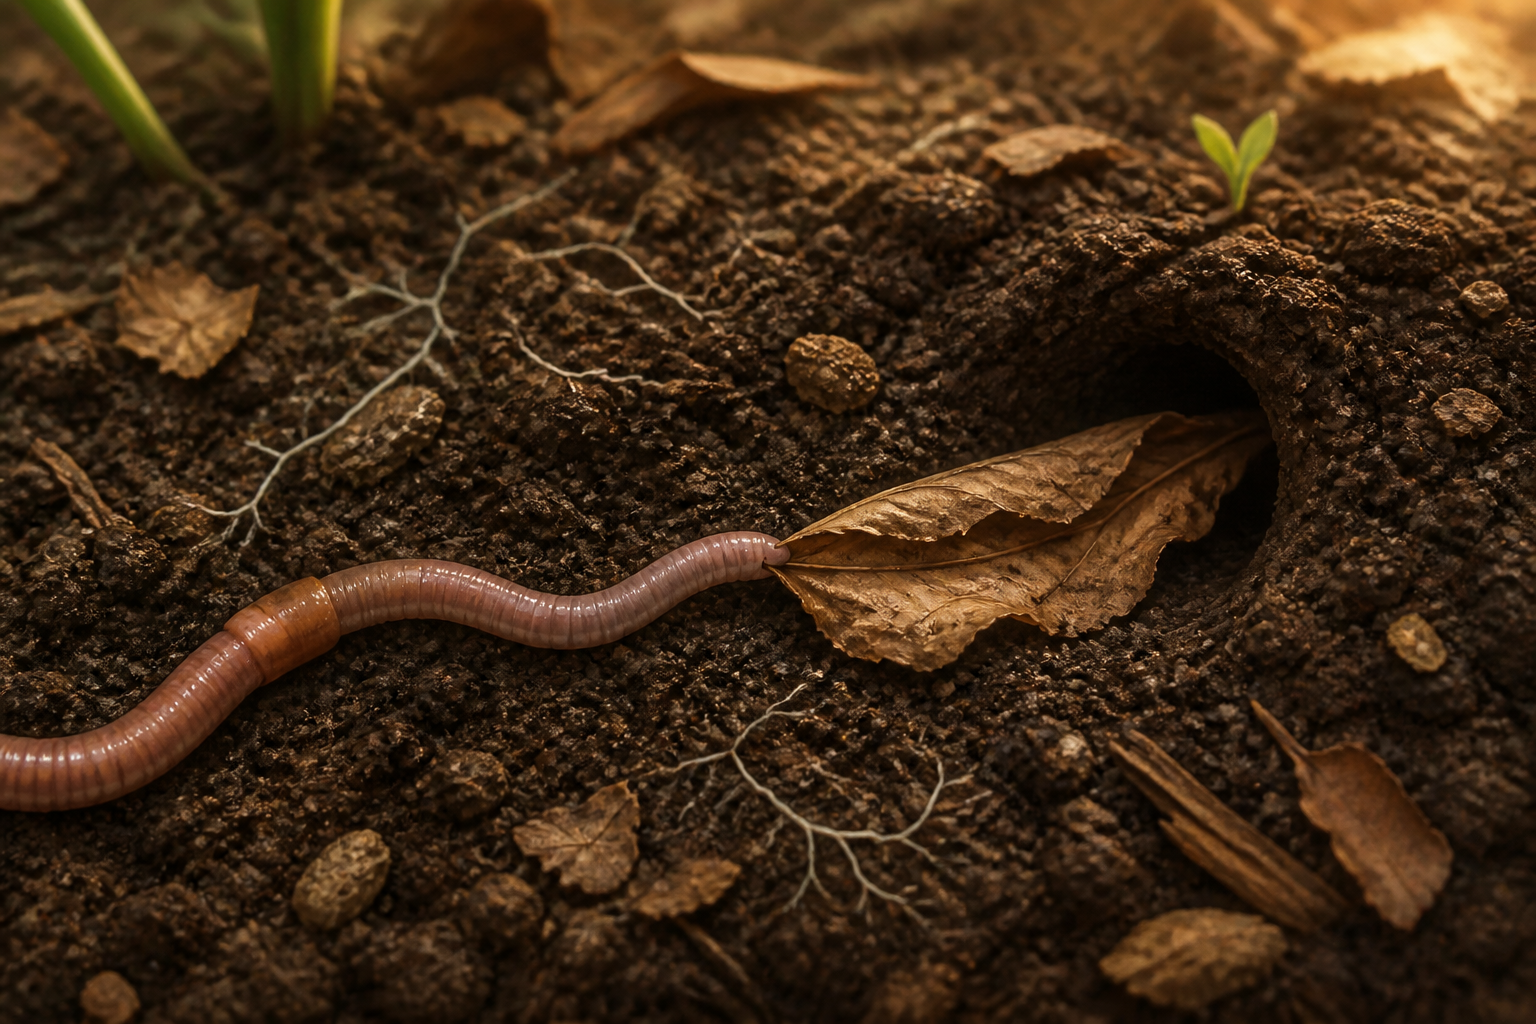
\includegraphics[width=0.6\linewidth]{images/book1/ai/g6-soil-earthworm.png}

{\small La fabricante de las tierras de labor, en plena faena: una \omterm{def:g1:plants-around-us:parts}{hoja}
camino del subsuelo y los hilos blancos de los \omterm{def:g6:decomposers-and-soil:decomposers}{hongos} ya minando las
demás.}
\end{omfigure}

\section{Ejercicios}

\begin{exercise}[$\star$]\label{exo:g6:decomposers-and-soil:1}
¿De qué está hecho el \omterm{def:g6:decomposers-and-soil:soil}{suelo}? Nombra sus cuatro ingredientes no vivos y
su preciada capa oscura.
\end{exercise}

\begin{exercise}[$\star$]\label{exo:g6:decomposers-and-soil:2}
¿De qué se alimentan los \omterm{def:g6:decomposers-and-soil:decomposers}{descomponedores}? Nombra cuatro visibles y uno
cuyo cuerpo de alimentarse sea un fieltro de hilos.
\end{exercise}

\begin{exercise}[$\star$]\label{exo:g6:decomposers-and-soil:3}
Enuncia en qué convierte la \omterm{prop:g6:decomposers-and-soil:decomposition}{descomposición} a la \omterm{def:g6:plants-are-producers:matter}{materia orgánica} --- y
el oficio de quién invierte con ello.
\end{exercise}

\begin{exercise}[$\star$]\label{exo:g6:decomposers-and-soil:4}
Vuelve a contar el último año de la \omterm{def:g1:plants-around-us:parts}{hoja} de roble en cuatro estaciones.
\end{exercise}

\begin{exercise}[$\star$]\label{exo:g6:decomposers-and-soil:5}
¿Por qué no se amontona año tras año la alfombra de otoño del bosque?
\end{exercise}

\begin{exercise}[$\star$]\label{exo:g6:decomposers-and-soil:6}
¿Con qué tres \omterm{def:g6:exploring-our-environment:conditions}{condiciones} trabajan más deprisa los \omterm{def:g6:decomposers-and-soil:decomposers}{descomponedores}? ¿En
qué parte del año se frena el trabajo y por qué?
\end{exercise}

\begin{exercise}[$\star\star$]\label{exo:g6:decomposers-and-soil:7}
Dibuja o describe el ciclo de la materia con sus tres oficios ---
\omterm{def:g5:food-webs:roles}{productoras}, \omterm{def:g5:food-webs:roles}{consumidores}, \omterm{def:g6:decomposers-and-soil:decomposers}{descomponedores} --- y una flecha entre cada
dos.
\end{exercise}

\begin{exercise}[$\star\star$]\label{exo:g6:decomposers-and-soil:8}
Explica el cubo de compost como un taller de \omterm{def:g6:decomposers-and-soil:decomposers}{descomponedores}: quién
trabaja allí, sobre qué, y qué produce para la huerta --- y ¿por qué
está caliente el montón?
\end{exercise}

\begin{exercise}[$\star\star$]\label{exo:g6:decomposers-and-soil:9}
Da los dos trabajos de la lombriz y di por qué los naturalistas
antiguos la llamaban la fabricante de las tierras de labor.
\end{exercise}

\begin{exercise}[$\star\star$]\label{exo:g6:decomposers-and-soil:10}
Pásale el \cref{met:g6:decomposers-and-soil:read} a dos \omterm{def:g6:decomposers-and-soil:soil}{suelos}: un
bancal acolchado y un sendero desnudo y pisoteado. Predice los
hallazgos de cada paso.
\end{exercise}

\begin{exercise}[$\star\star$]\label{exo:g6:decomposers-and-soil:11}
Una bolsa de plástico cerrada con recortes de césped se convierte en un
lodo apestoso en vez de en compost. ¿Qué condición de trabajo se le
negó, según la \cref{prop:g6:decomposers-and-soil:speed}, y qué
cambiaría el hortelano?
\end{exercise}

\begin{exercise}[$\star\star\star$]\label{exo:g6:decomposers-and-soil:12}
``Sin \omterm{def:g6:decomposers-and-soil:decomposers}{descomponedores}, las \omterm{def:g5:food-webs:roles}{productoras} se morirían de hambre entre
montañas de muertos''. Justifica las dos mitades de la frase con el
ciclo de la materia --- ¿qué se amontona y qué se acaba?
\end{exercise}

\section{Problema: Los experimentos de las bolsas de hojas}

\begin{problem}[{Problema de fin de semana --- bolsas de malla, hojas
enterradas y un invierno de ciencia del suelo}]\label{pb:g6:decomposers-and-soil:1}
La clase entierra bolsas de \omterm{def:g1:plants-around-us:parts}{hojas} en el talud del seto del colegio en
noviembre: pesos iguales de \omterm{def:g1:plants-around-us:parts}{hojas} frescas de roble en bolsas de malla,
para desenterrarlas y volver a pesarlas a lo largo del año. Tres tipos
de bolsa: malla gruesa (deja entrar lombrices, cochinillas, todo),
malla fina (excluye a la cuadrilla visible y solo admite a los
invisibles) y plástico sellado (excluye a todos y además al aire).

\medskip\noindent\textbf{Parte I --- El montaje.}
\begin{enumerate}
  \item ¿Por qué tienen que llevar todas las bolsas el \emph{mismo}
        peso de las \emph{mismas} \omterm{def:g1:plants-around-us:parts}{hojas}, enterradas el \emph{mismo}
        día en el \emph{mismo} talud? Nombra el método.
  \item ¿Qué pregunta hace la bolsa de malla fina que la de malla
        gruesa no puede hacer por sí sola?
  \item Un equipo quiere una cuarta bolsa: de malla gruesa, pero
        enterrada en la grava seca del patio. ¿Qué pregunta haría,
        según la \cref{prop:g6:decomposers-and-soil:speed}?
  \item Predice, antes de cavar: ordena las tres bolsas del talud según
        cuánto peso de \omterm{def:g1:plants-around-us:parts}{hoja} habrán perdido en junio.
\end{enumerate}

\medskip\noindent\textbf{Parte II --- Los resultados.}
\begin{enumerate}[resume]
  \item Las pesadas de junio: malla gruesa --- casi todo el peso
        desaparecido, \omterm{def:g1:plants-around-us:parts}{hojas} reducidas a \omterm{def:g3:bones-and-muscles:skeleton}{esqueletos} y migas; malla fina
        --- claramente aligerada, \omterm{def:g1:plants-around-us:parts}{hojas} reblandecidas y ennegrecidas
        pero más lenta; plástico sellado --- peso casi sin cambios y
        contenido convertido en lodo agrio. Interpreta cada bolsa.
  \item En la bolsa gruesa la clase encuentra cochinillas, una lombriz,
        colémbolos e hilos blancos de \omterm{def:g6:decomposers-and-soil:decomposers}{hongo}. Asigna a cada uno su papel
        en el desmontaje de la \omterm{def:g1:plants-around-us:parts}{hoja} (el modelo es el
        \cref{ex:g6:decomposers-and-soil:leaf}).
  \item La bolsa fina perdió peso de verdad aunque se excluyó a todos
        los \omterm{def:g1:animals-around-us:animal}{animales} visibles. ¿Qué demuestra eso sobre la vida
        invisible del \omterm{def:g6:decomposers-and-soil:soil}{suelo}?
  \item La bolsa de la grava del patio (la de la pregunta 3) perdió
        mucho menos que su gemela del talud. ¿Qué \omterm{def:g6:exploring-our-environment:conditions}{condiciones} de
        trabajo niega la grava?
\end{enumerate}

\medskip\noindent\textbf{Parte III --- La lección más amplia.}
\begin{enumerate}[resume]
  \item ¿Adónde \emph{se fue} el peso perdido de la bolsa gruesa?
        Responde con la
        \cref{prop:g6:decomposers-and-soil:decomposition} --- al menos
        dos destinos.
  \item Las ortigas de primavera del seto crecen más verdes justo a lo
        largo del talud donde la clase enterró sus bolsas. ¿Casualidad?
        Argumenta a partir del ciclo de la materia.
  \item Usa la bolsa sellada para explicar por qué los residuos
        orgánicos de un vertedero, envueltos herméticamente en
        plástico, aguantan décadas mientras que esos mismos residuos se
        compostan en unos meses.
  \item Concluye en dos frases: ¿qué demostró el invierno sobre quién
        despeja la alfombra del bosque y a quién alimenta ese despeje?
\end{enumerate}
\end{problem}
